\section{Traceability}
Traceability is important in every project and ours are not an exception. To assure traceability we have created a traceability matrix where all the Stakeholders Needs, User Stories, Acceptance Criteria and Test IDs are listed. In this way, we are always able to trace a test all the way back to the need of the stakeholder. \\
\\
In Scrum you usually write the user stories on a little piece of paper or a "Post-it"-note. Because of this, we have chosen to represent all the user stories with "User Story Cards". All user stories are listeed later in this document.  \\
\\
In this section we will elaborate how the Traceability Matrix is made and what it includes.

\subsection{Needs}
Defining and retrieving stakeholder needs are a crucial part of all project. All our User Stories can be traced back to the original need of the customer. Becuase of this, when we test something later in the project, we are able to say which stakeholder need we are accomplishing. This assures traceability for us and our stakeholders. The need section (Figure \ref{fig:needs} ) of our Traceability Matrix contains all the stakeholder needs we have identified in our project with the concern of the stakeholder and the uniqe ID of the need. 

\begin{figure}[h]
    \centering
        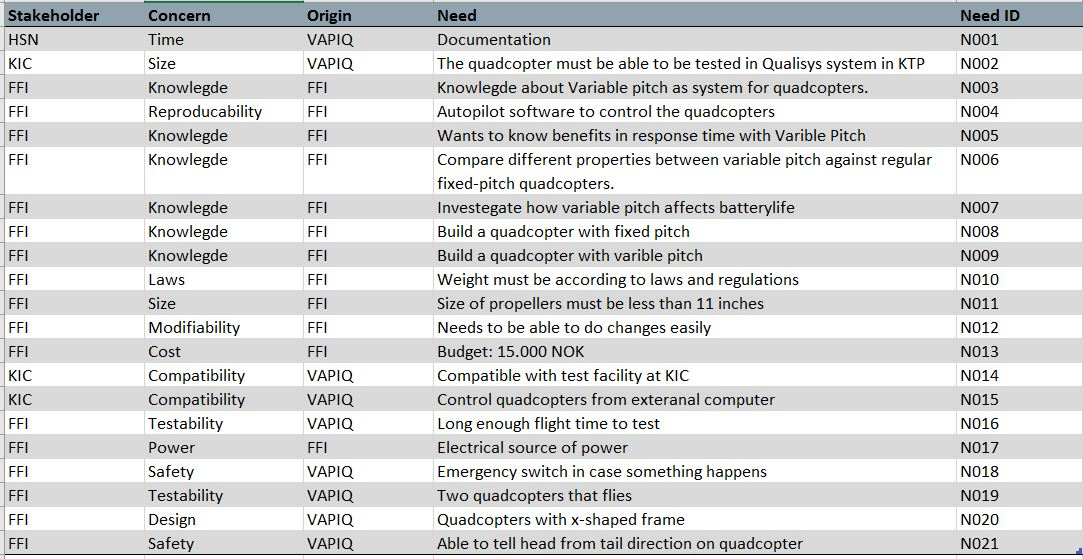
\includegraphics[width = 1\textwidth]{VAPIQ-PICTURES/Needs}
    \caption{Extraction of Needs}
    \label{fig:needs}
\end{figure}
\newpage

%%%% Backlog Matrix
\subsection{Backlog Matrix}
Our Product Backlog is represented in a Backlog Matrix (Figure \ref{fig:backlog}) where all user stories gets its own uniqe ID called BL ID. The Backlog Matrix links all the user stories with its corresponding Acceptance Criterion and Need ID. This is done because we want to be able to trace everything we do all the way back to what the customer wants. Every story is linked to an \textbf{Epic}. An Epic is a User Story that is too big to be done in one Sprint. Our project contains some main Epics and all of our user stories falls under one of these Epics. 

\begin{table}[h]
\begin{center}
\caption{List of Epics}
\begin{tabular}{l|l}
     \rowcolor{cadetgrey} \textbf{Epic Name:}      & \textbf{Jira ID:} \\
                        Mechanical Design                       & VPQ-1 \\  
\rowcolor{gainsboro}    Flight Controller - Software            & VPQ-2 \\  
                        Electro-Mechanical Design               & VPQ-3 \\  
\rowcolor{gainsboro}    Flight Controller - Control System      & VPQ-4 \\  
                        Communication                           & VPQ-5 \\  
\rowcolor{gainsboro}    Comparison                              & VPQ-6 \\  
                        Documentation                           & VPQ-7 \\  
\rowcolor{gainsboro}    Qualisys                                & VPQ-8 \\ 
                           
\end{tabular}
\end{center}
\end{table}
\\ 
\noindent The Backlog Matrix also includes information about which Sprint the given User Story was treated in and what the status of the story is. This status will only change when testing is done.  

\begin{figure}[h]
    \centering
        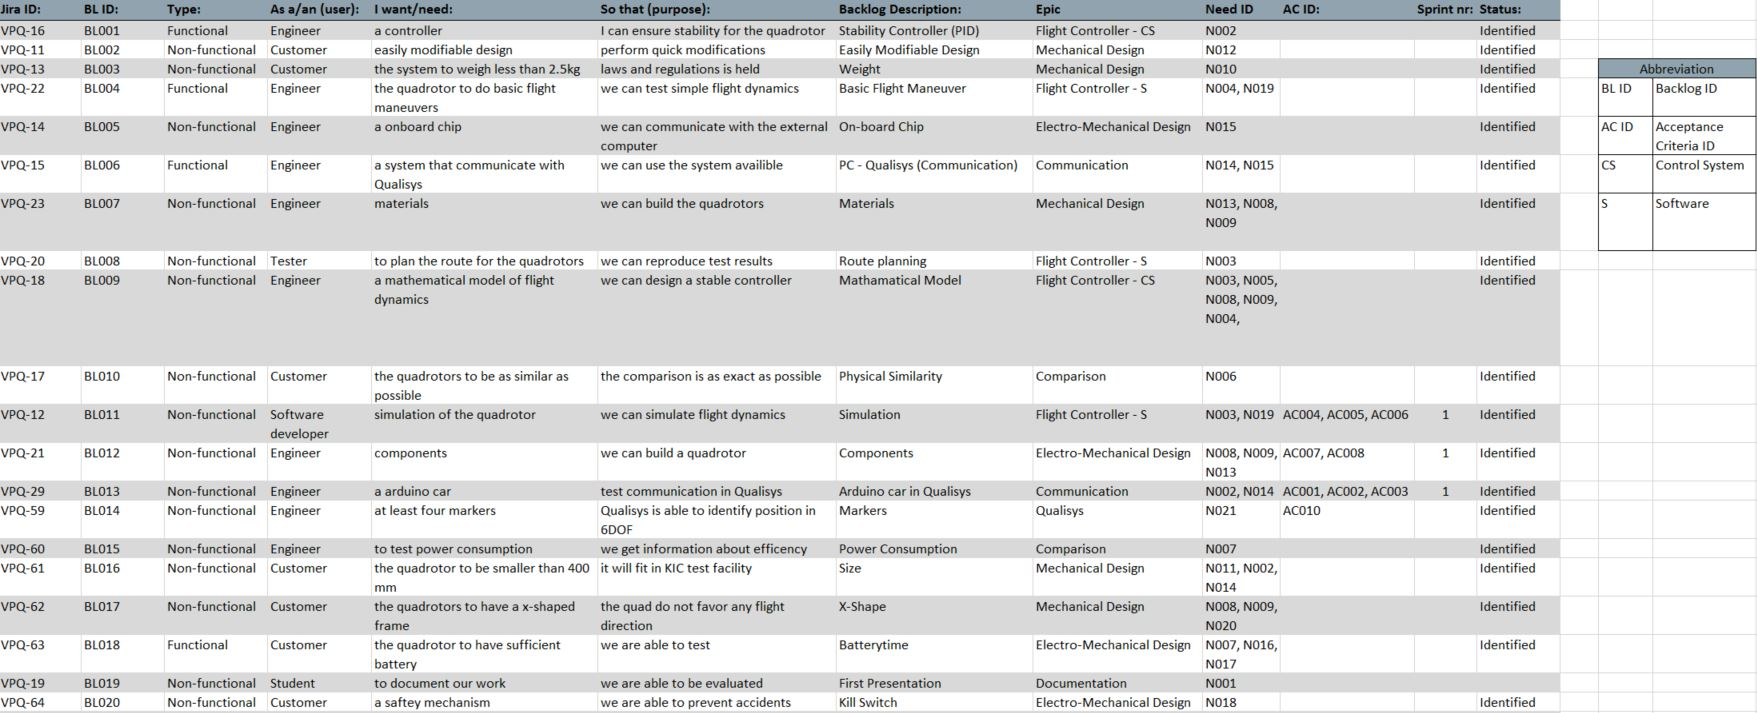
\includegraphics[width = 1\textwidth]{VAPIQ-PICTURES/BacklogMatrix}
    \caption{Extraction of the BacklogMatrix}
    \label{fig:backlog}
\end{figure}

\newpage

\subsection{Acceptance Criteria Matrix}
In the Acceptance Criteria section of the Traceability Matrix(Figure:\ref{fig:acm}) we list every Acceptance Criteria with the corresponding Backlog ID it is supposed to test. Every Acceptance Criteria get a uniqe ID named AC ID with the syntax AC000. 
\begin{figure}[h]
    \centering
        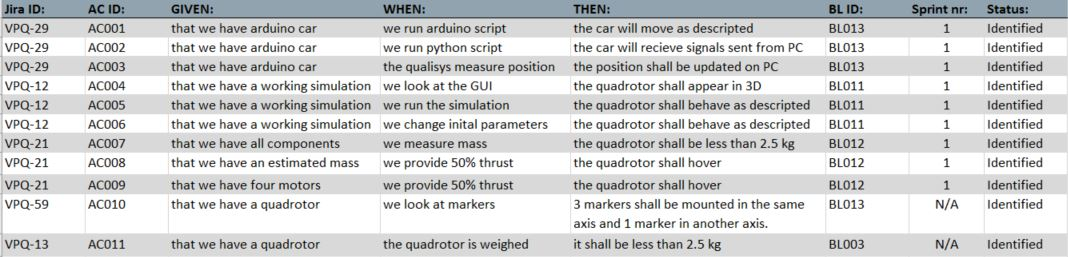
\includegraphics[width = 1\textwidth]{VAPIQ-PICTURES/AC}
    \caption{Extraction of Acceptance Criteria}
    \label{fig:acm}
\end{figure}

\newpage

\subsection{User Story Cards}
All of our Backlog Items, the user stories, are represented with "User Story Cards". These card are supposed to represent the more traditional "User Story Card" often written on paper. As mentioned earlier, user stories are written from the perspective of the end user and often with the customer in mind. The syntax is "As a/an, I want/need, So that". All our "Requirements" derived from the stakeholder needs are written in this form. \\ 
\\
This is the template for the User Story cards 

\krav{}{}{}{}{}{}{}


\noindent \textbf{BL ID} is our Backlog ID for the backlog item, this is created in the Traceability Matrix \\ \\
\textbf{Need ID} is the uniqe ID of the customer- or stakeholder need that the User Story are derived from. The needs can be found in the "Need" section of the Traceability Matrix \\ \\
\textbf{Jira ID} is the automatic ID the user story gets when created in Jira. As mentioned, all of our tasks and stories are numbered with a Jira ID starting with VPQ (Variable Pithc Quadcopter). This ID is uniqe and only used in Jira. This assures traceability between our manual Backlog and our Jira Backlog. \\ \\
\textbf{AC ID} is the ID of the Acceptance Criterion created for the user story. One user story may have multiple Acceptance Criteria.  \\
\textbf{Test ID} is the ID for the test linked to the user story. \\ \\
\textbf{Sprint} is the number of the Sprint where the User Story were treated. \\ \\
\textbf{User Story} includes the whole user story \\
\\
